\def\pgfsysdriver{pgfsys-dvisvgm.def}
\documentclass[tikz,border=4pt]{standalone}
\usepackage{amsmath}
\usetikzlibrary{calc}
% Semantic palette shared by the light and dark exports; geometry and TeX glyphs stay identical.
\ifdefined\FigureDark
  \definecolor{FigureForeground}{HTML}{E1E8DF}
  \definecolor{FigureMuted}{HTML}{94A69B}
  \definecolor{FigureBlue}{HTML}{8CC5F2}
  \definecolor{FigureOrange}{HTML}{F4B76B}
  \definecolor{FigureRed}{HTML}{F28E86}
  \definecolor{FigureBlueFill}{HTML}{273F4F}
  \definecolor{FigureOrangeFill}{HTML}{4A3726}
  \definecolor{FigurePaper}{HTML}{1B2420}
\else
  \definecolor{FigureForeground}{HTML}{202C29}
  \definecolor{FigureMuted}{HTML}{68766E}
  \definecolor{FigureBlue}{HTML}{245A88}
  \definecolor{FigureOrange}{HTML}{986000}
  \definecolor{FigureRed}{HTML}{A44030}
  \definecolor{FigureBlueFill}{HTML}{E5EDF8}
  \definecolor{FigureOrangeFill}{HTML}{FFF0D8}
  \definecolor{FigurePaper}{HTML}{FBFAF7}
\fi

\ifdefined\FigureDark
  \definecolor{FigureTeal}{HTML}{72D4BB}
\else
  \definecolor{FigureTeal}{HTML}{087462}
\fi
\begin{document}
% Intrinsic cut chart. The two wedge banks are exact, not a perspective view.
% Tip 1=(-1.45,-.15), banks 84/96 deg; tip 2=(1.45,-.15), banks 82/98 deg.
% Positive circuit crosses each right bank to its paired left bank.
% Seam maps are rotations +12 and +16 deg, giving chart vectors 30,42,58 deg.
% Color identifies transport stage in both the circuit and the comparison.
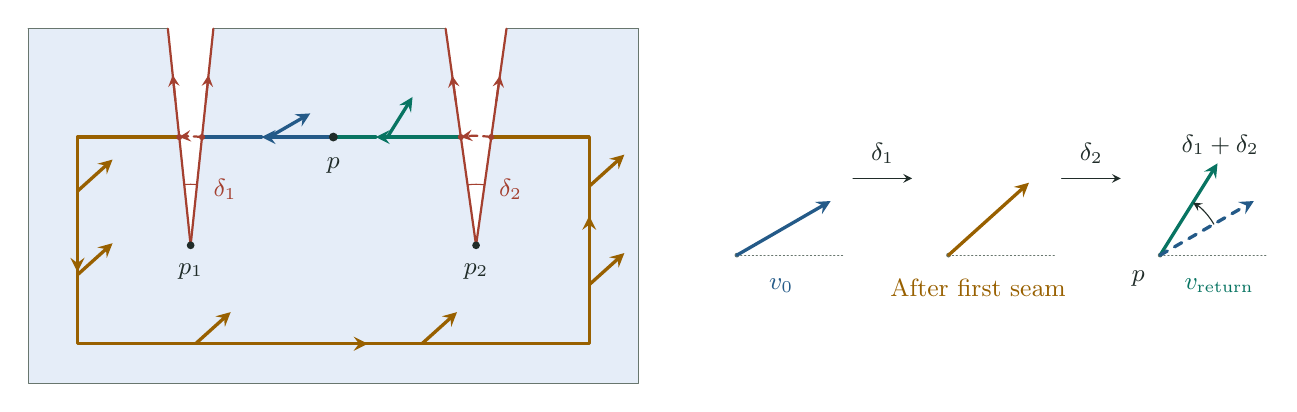
\begin{tikzpicture}[x=1.25cm,y=1.25cm,>=stealth,color=FigureForeground,
 font=\small,line cap=round,line join=round]
\coordinate (p1) at (-1.45,-.15); \coordinate (p2) at (1.45,-.15);
\coordinate (a1) at ({-1.45+1.1*tan(6)},.95);
\coordinate (b1) at ({-1.45-1.1*tan(6)},.95);
\coordinate (a2) at ({1.45+1.1*tan(8)},.95);
\coordinate (b2) at ({1.45-1.1*tan(8)},.95);
\coordinate (p) at (0,.95);
% The missing wedges reach the outer boundary; no extra surface bridges them.
\fill[FigureBlueFill] (-3.1,-1.55)--(3.1,-1.55)--(3.1,2.05)
 --({1.45+2.2*tan(8)},2.05)--(p2)--({1.45-2.2*tan(8)},2.05)
 --({-1.45+2.2*tan(6)},2.05)--(p1)--({-1.45-2.2*tan(6)},2.05)
 --(-3.1,2.05)--cycle;
\draw[FigureMuted] (-3.1,2.05)--(-3.1,-1.55)--(3.1,-1.55)--(3.1,2.05);
\draw[FigureMuted] (-3.1,2.05)--({-1.45-2.2*tan(6)},2.05)
 ({-1.45+2.2*tan(6)},2.05)--({1.45-2.2*tan(8)},2.05)
 ({1.45+2.2*tan(8)},2.05)--(3.1,2.05);
% Radial chevrons identify whole seam banks; dashed arcs identify the crossing.
\foreach \tip/\angle in {p1/84,p1/96,p2/82,p2/98}{
 \draw[FigureRed,thick] (\tip)--++(\angle:{2.2/sin(\angle)});
 \draw[FigureRed,thick,->] ($(\tip)+(\angle:1.48)$)--++(\angle:.26);
}
\draw[FigureRed] ($(p1)+(84:.62)$) arc(84:96:.62);
\draw[FigureRed] ($(p2)+(82:.62)$) arc(82:98:.62);
\node[FigureRed] at (-1.10,.42) {$\delta_1$};
\node[FigureRed] at (1.80,.42) {$\delta_2$};
\fill (p1) circle(1.4pt); \fill (p2) circle(1.4pt);
\node[below=3pt] at (p1) {$p_1$}; \node[below=3pt] at (p2) {$p_2$};
% Three connected transport stages in the quotient, separated at the seams.
\draw[FigureBlue,very thick,->] (p)--(-.73,.95);
\draw[FigureBlue,very thick] (-.73,.95)--(a1);
\draw[FigureOrange,very thick] (b1)--(-2.6,.95)--(-2.6,-1.15)
 --(2.6,-1.15)--(2.6,.95)--(a2);
\draw[FigureOrange,very thick,->] (-2.6,.15)--(-2.6,-.42);
\draw[FigureOrange,very thick,->] (-.4,-1.15)--(.35,-1.15);
\draw[FigureOrange,very thick,->] (2.6,-.45)--(2.6,.15);
\draw[FigureTeal,very thick,->] (b2)--(.43,.95);
\draw[FigureTeal,very thick] (.43,.95)--(p);
\draw[FigureRed,densely dashed,->,thick]
 (a1) arc(84:96:{1.1/cos(6)});
\draw[FigureRed,densely dashed,->,thick]
 (a2) arc(82:98:{1.1/cos(8)});
\foreach \q in {a1,b1,a2,b2}{\fill[FigureRed] (\q) circle(1.1pt);}
% Repeated equal vectors expose parallel transport along every flat path piece.
\foreach \x in {-.65}
  \draw[->,very thick,FigureBlue] (\x,.95)--++(30:.48);
\foreach \y in {.40,-.45}
  \draw[->,very thick,FigureOrange] (-2.6,\y)--++(42:.48);
\foreach \x in {-1.40,.90}
  \draw[->,very thick,FigureOrange] (\x,-1.15)--++(42:.48);
\foreach \y in {-.55,.45}
  \draw[->,very thick,FigureOrange] (2.6,\y)--++(42:.48);
\foreach \x in {.55}
  \draw[->,very thick,FigureTeal] (\x,.95)--++(58:.48);
\fill (p) circle(1.6pt); \node[below=4pt] at (p) {$p$};
% The comparison belongs to the final state, rather than a separate repeated panel.
\ifdefined\FigureStacked
  \def\StateX{-2.35}\def\StateY{-3.15}
\else
  \def\StateX{4.10}\def\StateY{-.25}
\fi
\begin{scope}[shift={(\StateX,\StateY)}]
\foreach \x in {0,2.15,4.30}{
 \draw[FigureMuted,densely dotted] (\x,0)--++(1.10,0);
 \fill[FigureMuted] (\x,0) circle(.85pt);
}
\draw[->,very thick,FigureBlue] (0,0)--++(30:1.10);
\draw[->,very thick,FigureOrange] (2.15,0)--++(42:1.10);
\draw[->,very thick,FigureTeal] (4.30,0)--++(58:1.10);
\draw[->,very thick,FigureBlue,dashed] (4.30,0)--++(30:1.10);
\draw[->,FigureForeground] ($(4.30,0)+(30:.63)$) arc(30:58:.63);
\draw[->,FigureForeground] (1.18,.78)--(1.78,.78);
\node[above=2pt] at (1.48,.78) {$\delta_1$};
\draw[->,FigureForeground] (3.30,.78)--(3.90,.78);
\node[above=2pt] at (3.60,.78) {$\delta_2$};
\node[below=5pt,FigureBlue] at (.45,0) {$v_0$};
\node[below=5pt,FigureOrange] at (2.45,0) {After first seam};
\node[below=5pt,FigureTeal] at (4.90,0) {$v_{\mathrm{return}}$};
\node[below left=2pt] at (4.30,0) {$p$};
\node[anchor=west] at (4.42,1.12) {$\delta_1+\delta_2$};
\end{scope}
\end{tikzpicture}
\end{document}
